\documentclass{article}
\usepackage{amsmath}
\usepackage[utf8]{inputenc}
\usepackage[margin=2cm]{geometry} 
\usepackage{graphicx}
\usepackage{placeins}
\usepackage[skip=10pt plus1pt, indent=40pt]{parskip}
\usepackage{float}
\usepackage{booktabs}
\usepackage{multicol}
\usepackage{gensymb}
\usepackage{amsmath}
\usepackage{hyperref}
\hypersetup{
    colorlinks=true,
    linkcolor=blue,
    filecolor=blue,
    citecolor=black,
    urlcolor=cyan
    }

\begin{document}

\title{Pendolo fisico: analisi del periodo a diverse distanze del punto di sospensione dal centro di massa}
\author{Alessia Di Nino}
\date{Giugno 2023}
\maketitle

\section{Introduzione}

\subsection{Cenni teorici} 
Un qualunque oggetto fissato ad un determinato punto di sospensione, e soggetto alla forza di gravità, rappresenta un pendolo fisico. Quando il sistema viene spostato di un angolo $\theta$ dalla posizione di equilibrio, il pendolo inizia ad oscillare e il momento della forza rispetto al punto di sospensione vale: 

\begin{equation}
\label{eq:1}
    \tau = -mgdsin\theta
\end{equation}

\begin{figure} [h]
    \centering
    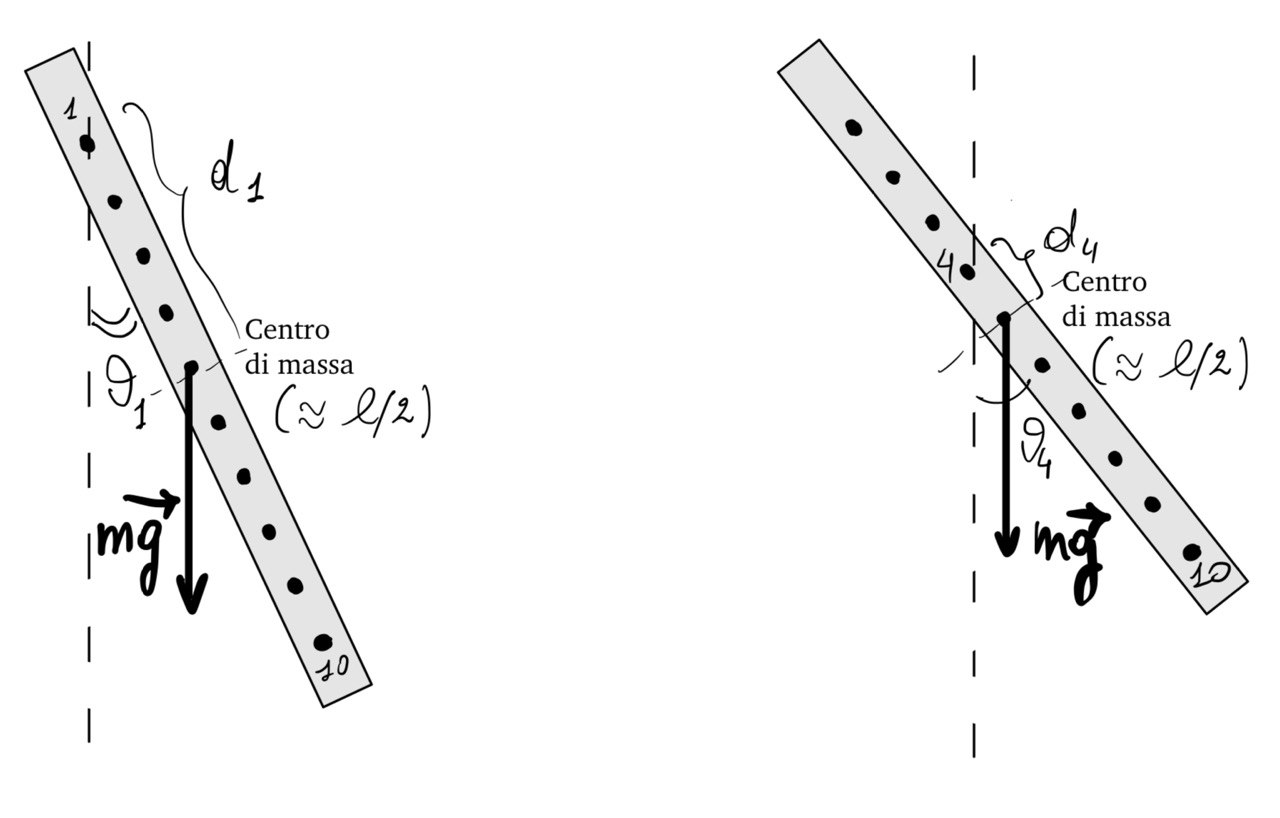
\includegraphics[width=15cm]{schema.jpg}
    \caption{schematizzazione delle grandezze e delle dimensioni in gioco}
    \label{fig:my_label}
\end{figure}

\FloatBarrier

Nello specifico caso di piccole oscillazioni possiamo considerare $sin\theta \sim \theta$. La condizione di "piccole oscillazioni" è quella in cui, dato un valore $\theta_0$,  si possano trascurare tutti i termini dello sviluppo in serie di Taylor superiori al primo $(T_0)$. 
% la condizione di piccole oscillazioni va verificata dopo che si è effettuata la misurazione e bisogna farlo per ogni tempo T0 misurato
\begin{equation}
    T(\theta_0) = T_0(1 + \frac{1}{16}\theta_0 ^2 + \frac{11}{3072} \theta_0 ^4 + \frac{173}{737280} \theta_0 ^6 + ...)
\end{equation}

Se vogliamo considerare le oscillazioni piccole, devo assicurarmi che i termini di correzione al periodo che trascuro siano dunque molto più piccoli dell'incertezza di misura sul periodo stesso.\\
In formule, vale a dire:
\begin{equation}
    \theta_0 << 4\sqrt\frac{\sigma_T}{T_0}
\end{equation}
Fatta questa approssimazione (che verificheremo nella descrizione delle misure) dunque, la \eqref{eq:1}
diventa:

\begin{equation}
    \label{eq:3}
    \tau = -mgd\theta
\end{equation}

Inoltre, per la seconda equazione cardinale si ha $\tau = \frac{dL}{dt}$, e sostituendo $L=I\omega$ e $\omega=\frac{d\theta}{dt}$ si ottiene:

\begin{equation}
    \label{eq:4}
    \tau = I\frac{d^2\theta}{dt^2}
\end{equation}
Con I momento di inerzia dell'asta, di massa m e lunghezza l, rispetto ad un punto P che dista d dal centro di massa. 

A questo punto, la \eqref{eq:3} e la \eqref{eq:4} consentono di scrivere l'equazione differenziale di un moto armonico:

\begin{equation}
    \frac{d^2\theta}{dt^2} + \frac{mgd\theta}{I} = 0
\end{equation}

Questo ha pulsazione regolare $\omega_0$ e periodo $T_0$ dati da:

\begin{equation}
    \omega_0 = \sqrt{\frac{mgd}{I}}
\end{equation}

\begin{equation}
    T_0 = \frac{2\pi}{\omega_0} = 2\pi\sqrt{\frac{I}{mgd}}
\end{equation}

Sapendo inoltre che 

\begin{equation}
    I = I_cm + md^2 = \frac{ml^2}{12} + md^2
\end{equation}

è allora possibile scrivere

\begin{equation}
    \label{eq:9}
    T(d) = 2\pi\sqrt{\frac{l^2/12 + d^2}{gd}}
\end{equation}

con l parametro libero.

\vspace{1em}

\subsection{Scopo dell'esperienza} 
Scopo dell'esperienza, infatti, è proprio eseguire un fit (con il modello espresso dalla \eqref{eq:9}) dei dati raccolti nella misurazione del periodo di oscillazione T (al variare della distanza d del punto di sospensione dal centro di massa) con l parametro libero, e confrontare il valore di best - fit di l con la lunghezza dell'asta misurata sperimentalmente.

\section{Metodi} 

\subsection{Apparato sperimentale} 
Per l'esperimento, ci siamo servite di:

\begin{itemize}
    \item asta rigida con 10 fori
    \item supporto di sospensione;
    \item calibro ventesimale di risoluzione 0.05 mm;
    \item metro a nastro di risoluzione 0.1cm;
    \item righello di risoluzione 0.1 cm;
    \item cronometro di risoluzione 0.01 s.
\end{itemize}
\vspace{1em}

\FloatBarrier

\begin{figure} [H]
    \centering
    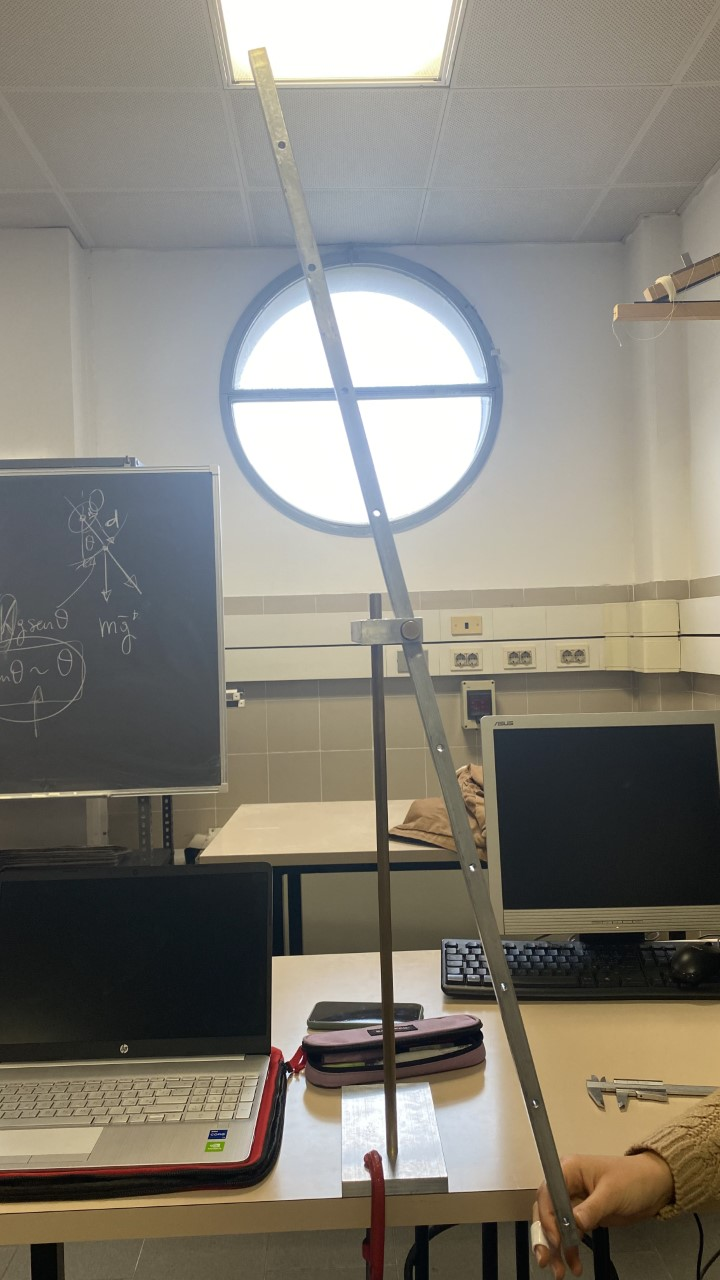
\includegraphics[width=8cm]{sbarra_forata.jpg}
    \caption{Asta rigida con 10 fori}
    \label{fig:my_label}
\end{figure}

\FloatBarrier

\begin{figure}
    \centering
    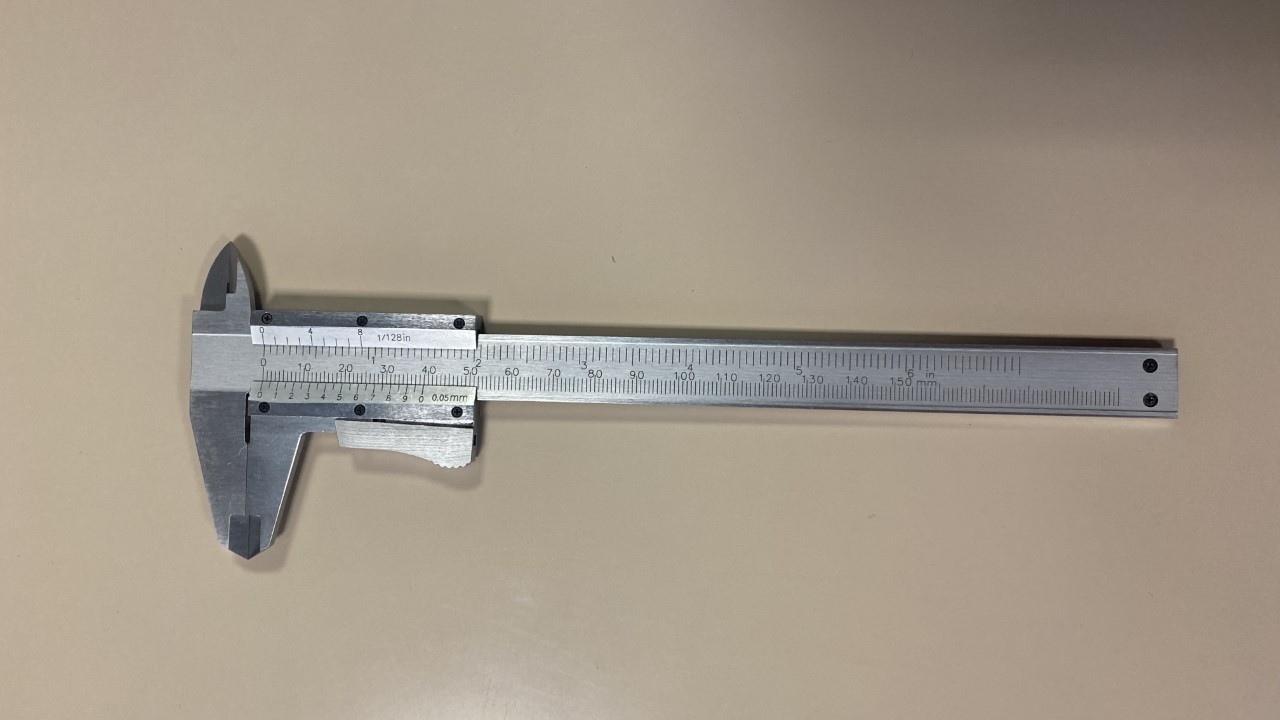
\includegraphics[width=9cm]{calibro.jpg}
    \caption{Calibro ventesimale}
    \label{fig:my_label}
\end{figure}

\begin{figure}
    \centering
    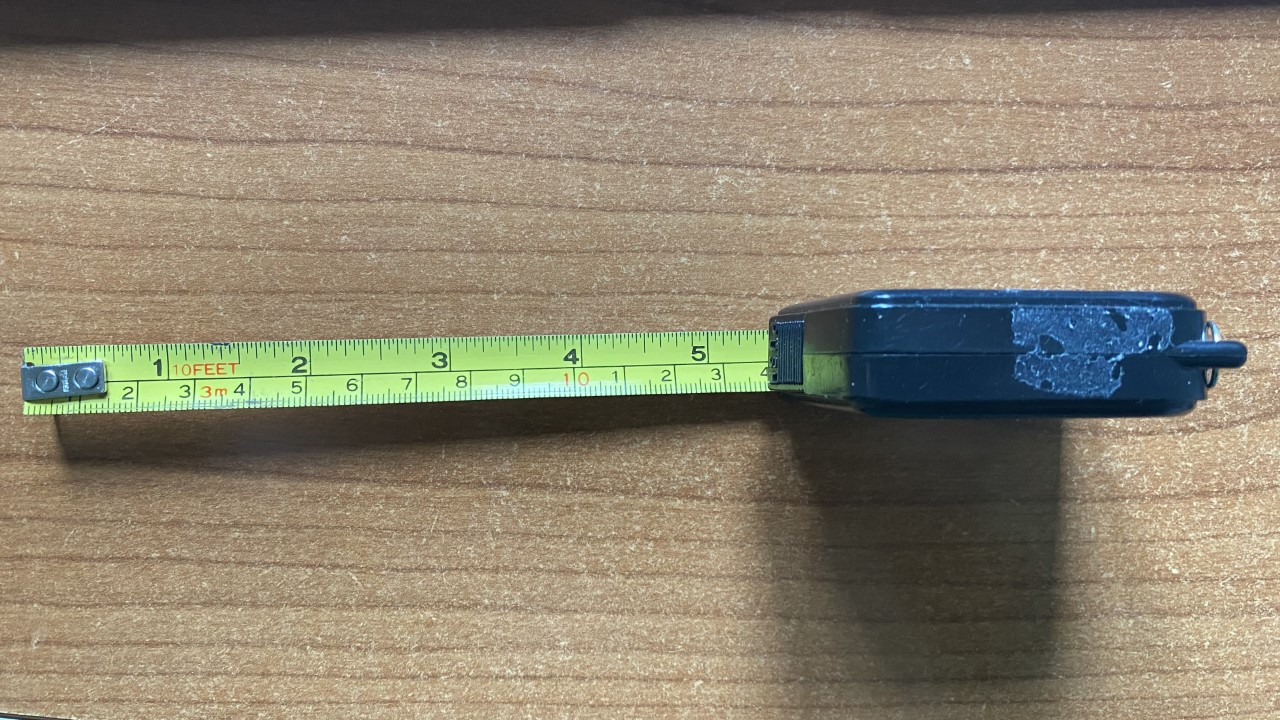
\includegraphics[width=9cm]{metro.jpg}
    \caption{Metro a nastro}
    \label{fig:my_label}
\end{figure}

\begin{figure}
    \centering
    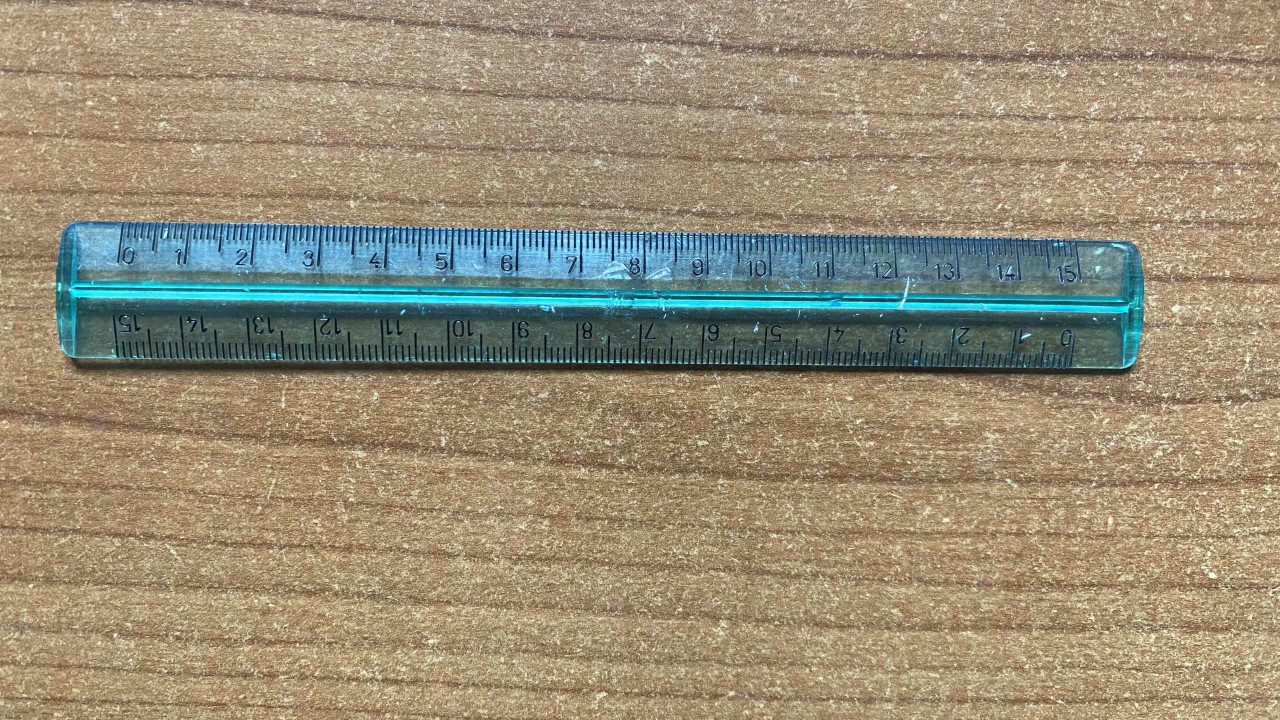
\includegraphics[width=9cm]{righello.jpg}
    \caption{Righello}
    \label{fig:my_label}
\end{figure}

\begin{figure}
    \centering
    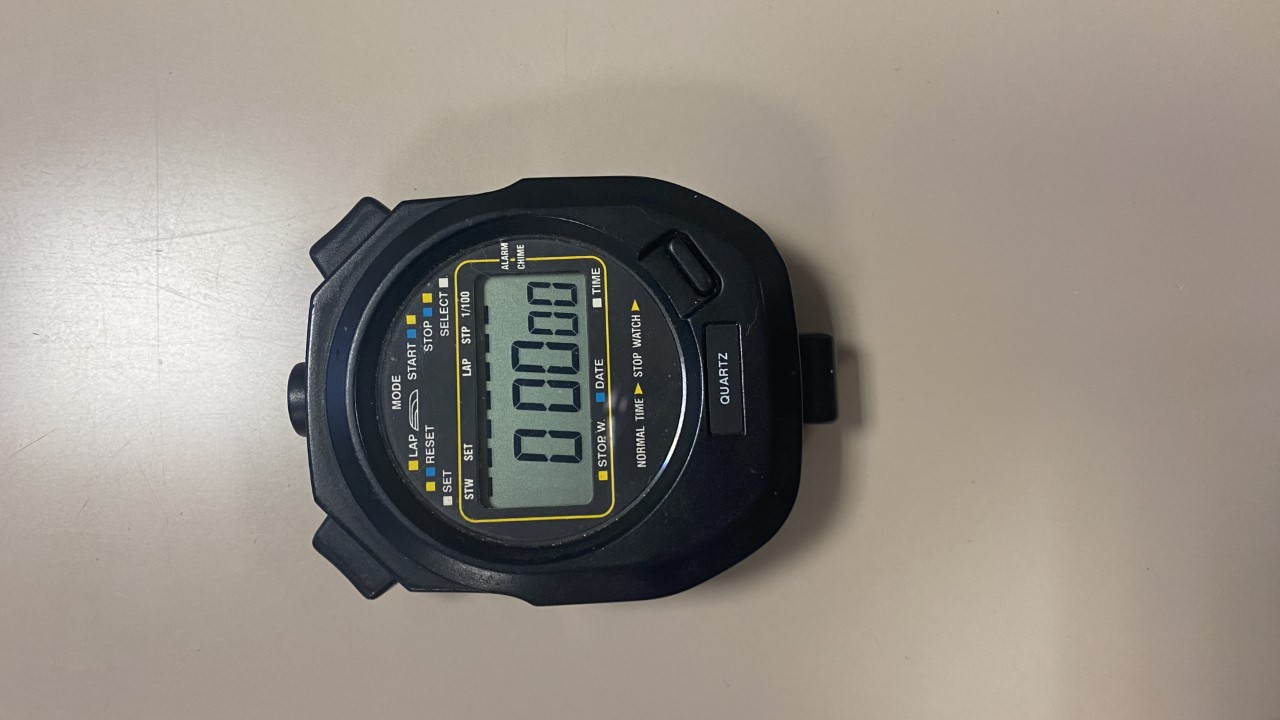
\includegraphics[width=9cm]{cronometro.jpg}
    \caption{Cronometro}
    \label{fig:my_label}
\end{figure}

\FloatBarrier

\subsection{Descrizione delle misure} 
\label{subsec: misure}
Abbiamo inizialmente misurato le dimensioni dell'asta e dei fori, così da condurre una serie di osservazioni sul centro di massa dell'asta stessa. Abbiamo utilizzato il metro a nastro per misurare la lunghezza dell'asta, il diametro dei fori e la distanza tra i fori e da questi agli estremi dell'asta, mentre abbiamo usato il calibro ventesimale per misurare la base dell'asta; abbiamo associato ad ogni misura l'incertezza pari alla risoluzione dello strumento utilizzato, ed abbiamo ottenuto i seguenti dati:

\begin{center}
    \begin{tabular}{c|c}
    \toprule
     $lunghezza dell'asta & (99.0 \pm 0.1) cm \\
     lato di base dell'asta & (15.70 \pm 0.05) mm \\
     diametro dei fori & (0.7 \pm 0.1) cm \\
     distanza foro 1 dall'estremo superiore & (8.0 \pm 0.1)cm \\
     distanza foro 2 dall'estremo inferiore & (2.0 \pm 0.1)cm \\
     distanza tra un foro e l'altro & (10.0 \pm 0.1)cm \\$
     \bottomrule
\end{tabular}
\end{center}

A questo punto, abbiamo notato che i fori erano sì equidistanti tra loro, ma il primo e l'ultimo non lo erano  dagli estremi dell'asta. Abbiamo pensato che questo potesse influire sulla posizione del centro di massa dell'asta, dato fondamentale per condurre tutte le successive misure, e abbiamo misurato le proporzioni in cui questo fenomeno potesse verificarsi. A questo fine, abbiamo misurato il volume dell'asta in ipotetica assenza di fori e il volume dei soli fori dell'asta (sfruttando le formule per il volume del parallelepipedo e per la propagazione dell'errore: $V = r^2 h$ e $\sigma_V = V \sqrt{\frac{4\sigma_r ^2}{r^2} + \frac{\sigma_h ^2}{h^2}$)

\begin{center}
\begin{tabular}{c|c}
    \toprule
    volume dell'asta senza fori  &  (61.66 \pm 0.84) cm^3 \\
    volume dei soli fori & (6.04 \pm 0.35) cm^3\\
    \bottomrule
\end{tabular}
\end{center}

Tramite la proporzione, abbiamo trovato che il volume dei fori rappresenta il 9.8\% del volume totale. Poichè i buchi sono spostati di $(2.0 \pm 0.1)cm$ rispetto al centro di massa, questo equivale in percentuale ad uno spostamento del centro di massa di 0.19 cm, ma siccome abbiamo misurato la posizione del centro di massa con un metro a nastro (di risoluzione pari a 0.1 cm) possiamo ritenere lo spostamento trascurabile e considerare il centro di massa nel punto aspettato, ossia a metà dell'asta.\\
\\
%oppure dobbiamo richiedere che la somma dei volumi dei fori sia molto più piccola dell'incertezza sul volume dell'intera asta
Per quanto riguarda le misure di tempo, esse sono state effettuate tramite cronometro manuale, ma per ridurre l'errore sui tempi di reazione di chi effettuava la misura, abbiamo fatto compiere al pendolo, per ogni foro, dieci oscillazioni complete e abbiamo ripetuto le misure sei volte per ogni foro; abbiamo poi preso il valor medio e la deviazione standard della media delle misure come miglior stima del misurando e relativa incertezza associata (calcolati tramite "cicli for" su python). Inoltre, per esser certe di poter sfruttare le leggi descritte in \ref{subsec: misure} per angoli piccoli (sotto i 20° in questo caso), abbiamo misurato l'angolo da cui facevamo partire l'oscillazione utilizzando righello e metro a nastro, sfruttando la relazione: $\alpha = arccos \frac{b}{a}$ (cfr. \ref{fig:angolo} )

\begin{figure} [H]
    \centering
    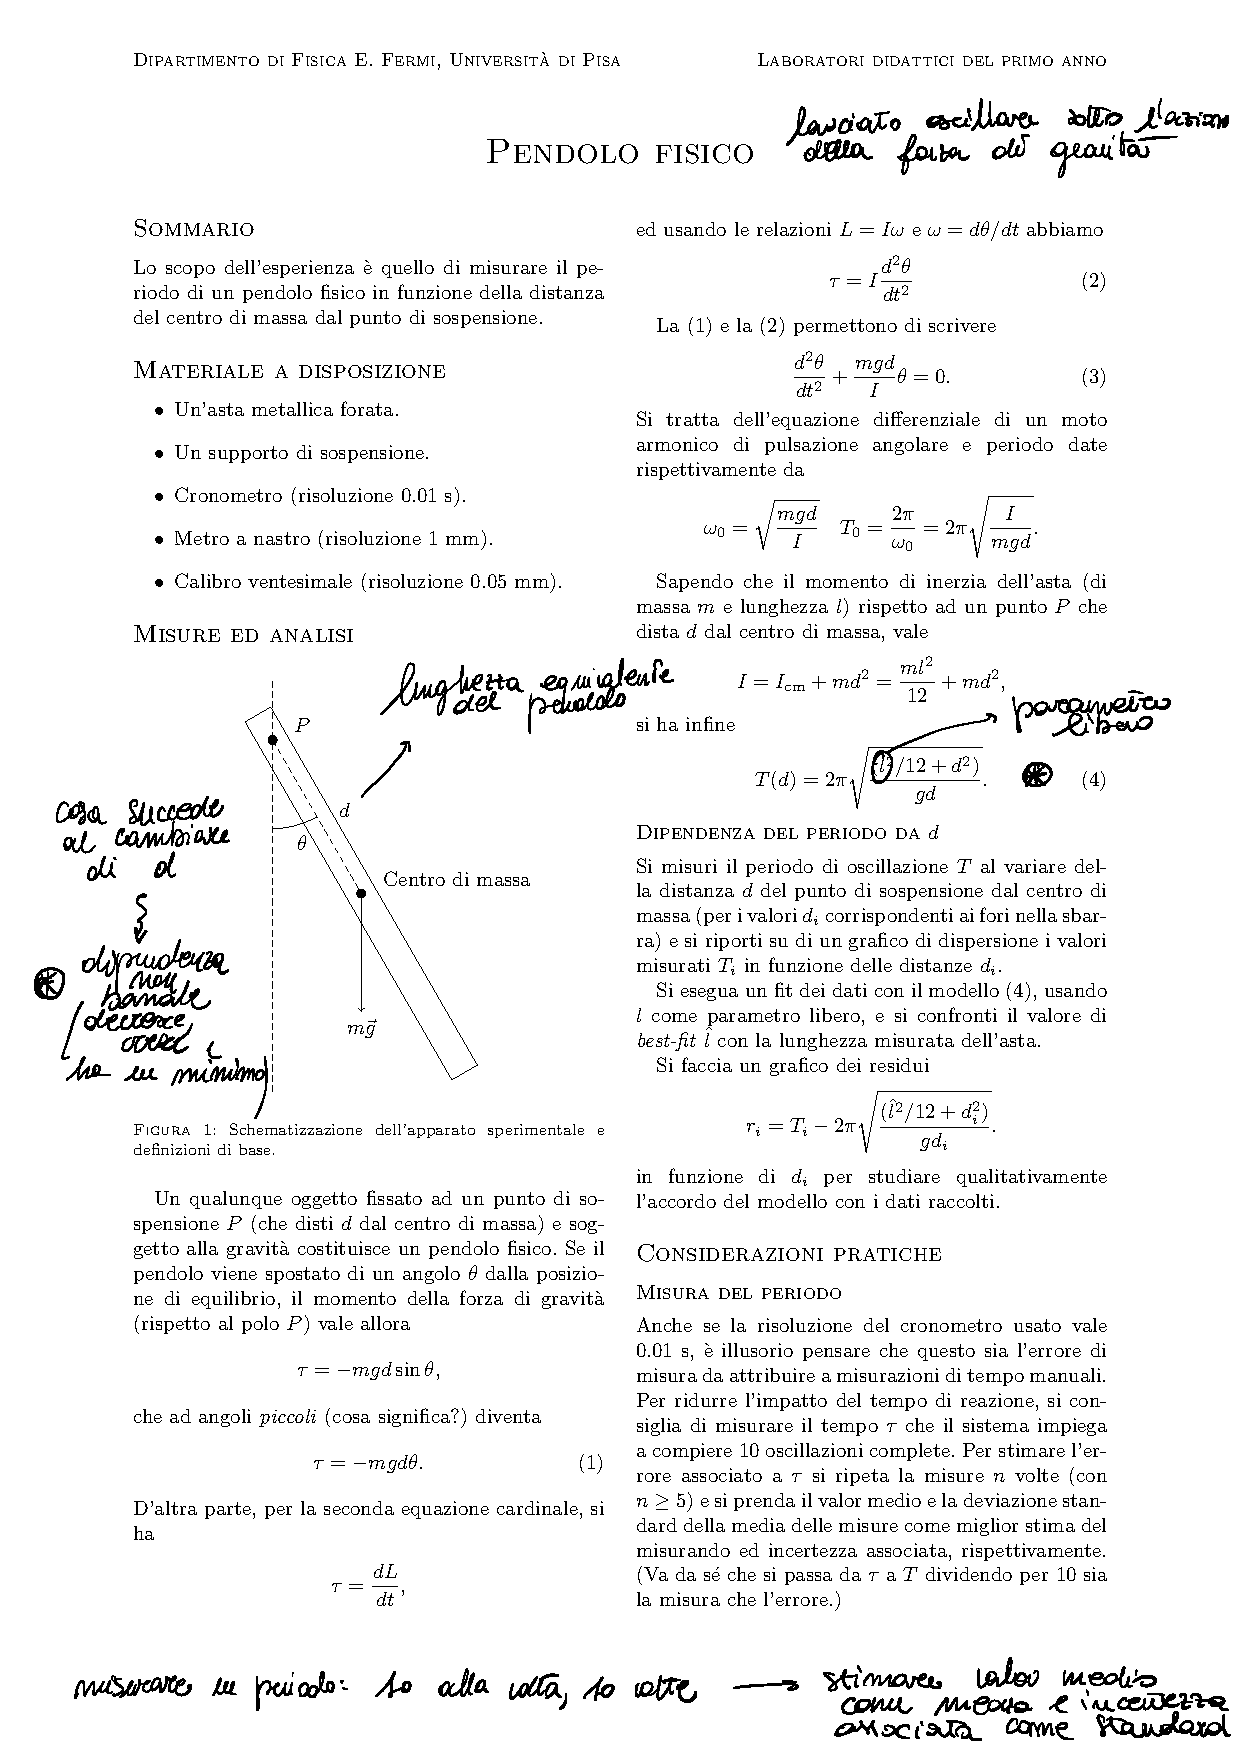
\includegraphics[width=8cm]{pendolo_fisico.pdf}
    \caption{Schematizzazione della misura dell'angolo}
    \label{fig:angolo}
\end{figure}

Di seguito, la tabella con i dati raccolti:

\begin{center}
\begin{tabular}{c|c}
    \toprule
    foro & periodo (s) \\
    \midrule
    1 &  1.57 \pm 0.02 \\
    2 & 1.53 \pm 0.07\\
    3 & 1.54 \pm 0.05\\
    4 & 1.81 \pm 0.06\\
    5 & 3.88 \pm 0.13\\
    6 & 2.16 \pm 0.08\\
    7 & 1.59 \pm 0.02\\
    8 & 1.51 \pm 0.03\\
    9 & 1.56 \pm 0.04\\
    10 & 1.63 \pm 0.03\\
    \bottomrule
\end{tabular}
\end{center}
%inserisci anche i dati
\vspace{1em}

\subsection{Analisi dei dati - metodo di fit e grafico dei residui condotto utilizzando la funzione curve\_fit() di Python} %5 - alessandra
I dati raccolti sono stati analizzati tramite la funzione curve\_fit() di Python, realizzando, per l'appunto, il grafico di best fit e il grafico dei residui.

\begin{figure} [H]
    \centering
    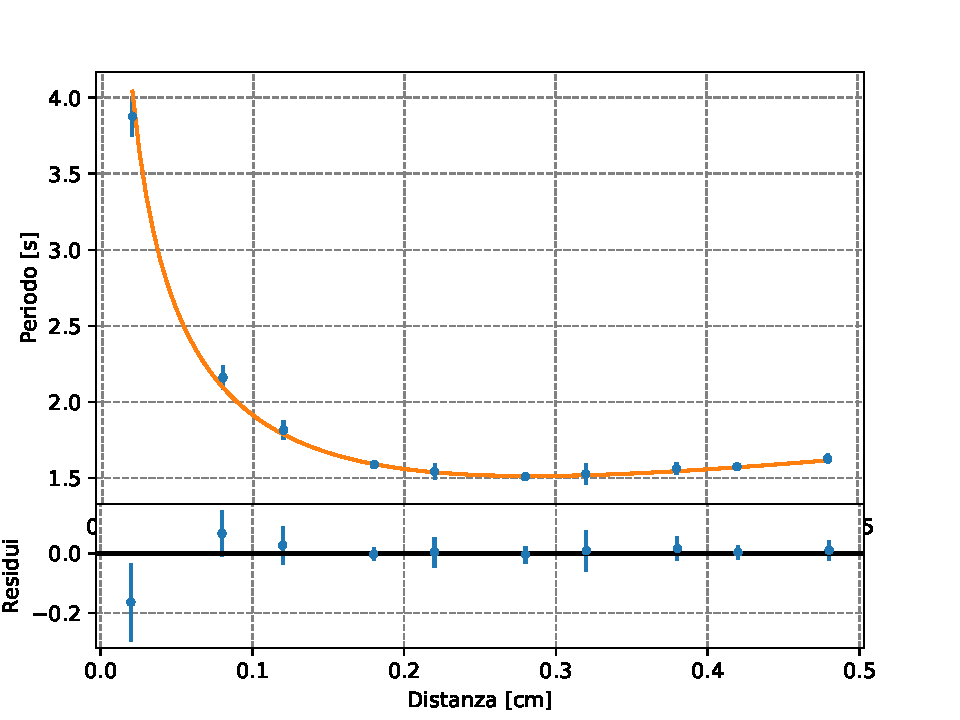
\includegraphics[width=15cm]{fit and residuals.pdf}
    \caption{Grafico di fit e residui}
    \label{fig:my_label}
\end{figure}

\FloatBarrier

\section{Conclusioni} %6 - alessia
Possiamo infine affermare che il modello di fit è corretto grazie a due commenti. Come osservazione preliminare, notiamo che i grafici dei residui mostrano che i valori oscillano attorno allo zero con fluttuazioni paragonabili alle barre d'errore considerate. \\
Inoltre, confrontando il valore di best fit di l con la lunghezza misurata dell'asta, viene fuori che si tratta di due misure compatibili:

\begin{center}
\begin{tabular}{c|c}
    \toprule
    parametro di best fit l & misura empirica di l \\
    \midrule
    (0.984 \pm 0.007)m & (0.990 \pm 0.001)m \\
    \bottomrule
\end{tabular}
\end{center}
%inserisci chi quadro

\end{document}
